\section{Processi organizzativi}

\subsection{Gestione di processo} \label{_gestioneDiProcesso}

\subsubsection{Scopo}
Secondo lo standard ISO-12207:1995 la gestione di processo contiene le attività e i compiti generici che vengono impiegati per gestire i vari processi.\\
Il Responsabile di progetto è responsabile della gestione del prodotto, del progetto, e delle attività o processi ad esso applicabili.
\subsubsection{Aspettative}
Le aspettative per questo processo sono:
\begin{itemize}
    \item coordinare e semplificare la comunicazione tra i membri del team, assegnando alle singole componenti ruoli e compiti da svolgere;
    \item avere il controllo sul progetto, monitorando il lavoro del team ed in che stato sono i compiti da svolgere;
    \item avere una buona pianificazione delle attività da seguire.
\end{itemize}

\subsubsection{Descrizione}
In questo processo discuteremo delle seguenti attività:
\begin{itemize}
    \item comunicazioni e riunioni tra i membri del gruppo;
    \item comunicazioni e riunioni con i proponenti e committenti;
    \item assegnazione dei ruoli e dei compiti;
    \item esecuzione e revisione di un compito;
    \item pianificazione di risorse, tempi e costi.
\end{itemize}

\subsubsection{Coordinamento} \label{_gestioneDiProcesso_coordinamento}
L'attività di coordinamento consente di gestire la comunicazione sia interna che esterna, e le riunioni. Ciò viene fatto attraverso comportamenti precisi che ogni membro del gruppo deve avere per l'intera durata del processo.

\paragraph{Comunicazioni}
Oltre che la comunicazione all'interno del gruppo (Comunicazione interna), durante lo sviluppo del progetto il team si troverà a comunicare con diversi attori esterni:
\begin{itemize}
    \item \textbf{proponente}: RedBabel;
    \item \textbf{committenti}: Prof. Tullio Vardanega e Prof. Riccardo Cardin;
    \item \textbf{competitor}: verranno valutati dopo la Revisione dei Requisiti.
\end{itemize}

\subparagraph{Comunicazione interna}
Viene utilizzata come piattaforma principale \glock{Slack} per comunicazioni che abbiano lo scopo di coordinamento o decisionale, mentre per comunicazioni meno importanti e più informali può essere utilizzato un gruppo \glock{Telegram}.
Le discussioni su Slack dovranno essere svolte all'interno del canale appropriato, e qual ora si ritenga necessario crearne uno nuovo va fatta segnalazione al Responsabile di progetto che provvederà a valutarne la creazione.\\
I canali di discussione sono organizzati nel seguente modo:
\begin{itemize}
    \item un canale per ogni documento dove si discute del contenuto dello stesso;
    \item \textbf{\#glossario}: per discutere ciò da aggiungere al glossario e delle relative definizioni;
    \item \textbf{\#scadenze}: per scrivere le scadenze future;
    \item \textbf{\#proponente}: discutere di argomenti che probabilmente avranno un coinvolgimento del proponente per porgli delle domande;
    \item \textbf{\#varie}: canale per avere comunicazioni di carattere generale.
\end{itemize}
Un'altra piattaforma di cui ci si avvale è Discord, la quale attraverso le chat vocali può essere utilizzata per svolgere dei compiti o attività con altri membri. In alternativa è possibile utilizzare \glock{Zoom}, in quanto applicazione utilizzata e conosciuta da tutto il team.

\subparagraph{Comunicazione esterna}
Il gruppo è provvisto di un indirizzo email che verrà utilizzato per comunicazioni esterne, in particolare per comunicazioni verso i committenti. Il controllo della casella di posta elettronica per verificare la presenza di nuove comunicazioni può essere svolto da qualunque membro del gruppo, mentre l'invio di una nuova email è effettuabile soltanto dal Responsabile di progetto.\\
Tutti i membri del team sono altresì presenti all'interno dello Slack del proponente. I canali in questo caso sono due:
\begin{itemize}
    \item \textbf{\#swe-2020\_2021}: canale di discussione in cui sono presenti anche gli altri gruppi che svolgono lo stesso capitolato;
    \item \textbf{\#swexception}: canale del gruppo in cui poter fare domande al proponente.
\end{itemize}

\paragraph{Riunioni}
Per ogni riunione, sia essa interna od esterna, verrà nominata una persona incaricata di prendere appunti e far rispettare l'ordine del giorno. Al termine della riunione avrà anche il compito di redarre il verbale e farlo avere agli altri membri entro breve tempo.

\subparagraph{Riunioni interne}
È consentita la partecipazione ai soli membri del team, e per essere svolta deve essere presente più del $50\%$ delle componenti del gruppo. Vengono svolte su una stanza Zoom creata appositamente, o in alternativa in caso di problemi su Discord in una chat vocale dedicata.

\subparagraph{Riunioni esterne}
Sono svolte con i proponenti o committenti, e si terranno su GMeet per riunioni con i proponenti e su Zoom per quelle con i committenti. Il link per il collegamento verrà comunicato dai soggetti esterni nel momento in cui si pianifica un incontro con essi.

\subsubsection{Pianificazione} \label{_gestioneDiProcesso_pianificazione}
Questa sezione ha lo scopo di definire come si intende pianificare il lavoro che c'è da svolgere, come vengono assegnati i compiti tra i membri del gruppo, e in cosa consistono i singoli ruoli.

\paragraph{Ruoli di progetto}
I ruoli, cioè le rispettive figure aziendali che ogni membro del gruppo deve coprire, saranno assegnati in modo tale che ognuno di essi sia stato ricoperto per un numero simile di ore da ogni componente del gruppo. Nel fare ciò bisognerà evitare conflitti di interesse, cioè un componente non potrà verificare un prodotto da lui stesso realizzato. \\
I ruoli che saranno ricoperti nel corso del progetto sono:
\begin{itemize}
    \item Responsabile di progetto;
    \item Amministratore di progetto;
    \item Analista;
    \item Progettista;
    \item Programmatore;
    \item Verificatore.
\end{itemize}

\subparagraph{Responsabile di progetto}
Il Responsabile di progetto è un ruolo fondamentale che deve essere ricoperto per l'intera durata del progetto. Il suo compito principale è coordinare il team e rappresentarlo verso l'esterno. \\
In particolare questo ruolo comporta:
\begin{itemize}
    \item responsabilità di scelte e approvazioni;
    \item responsabilità sulla pianificazione delle attività rispettando le scadenze;
    \item coordinare i membri del gruppo e i compiti da svolgere;
    \item controllare, coordinare e relazionarsi verso soggetti esterni;
    \item avere conoscenze e capacità per saper valutare rischi, scelte, alternative.
\end{itemize}

\subparagraph{Amministratore di progetto}
L'Amministratore di progetto è la figura che ha il controllo sull'ambiente di lavoro, pertanto il suo ruolo comporta i seguenti punti:
\begin{itemize}
    \item amministrare le infrastrutture e servizi di supporto;
    \item risolvere problemi legati alla gestione dei processi;
    \item salvaguardare la documentazione di progetto, controllando che venga verificata e corretta;
    \item controllare il versionamento e le configurazioni dei prodotti;
    \item individuare strumenti che portino ad una maggiore automazione dei processi.
\end{itemize}

\subparagraph{Analista}
L'Analista si occupa di studiare a pieno il problema comprendendone tutte le caratteristiche. Questo ruolo è fondamentale nella fase iniziale, in particolare nella stesura dell'Analisi dei Requisiti, in quanto errori o mancanze in questa fase potrebbe compromettere il risultato del progetto.\\
Si deve occupare di:
\begin{itemize}
    \item studiare il dominio del problema;
    \item analizzare e definire le richieste e quindi i requisiti del proponente, anche ciò che non è stato descritto esplicitamente;
    \item analizzare dove verrà applicato il prodotto finito, e quindi i relativi casi d'uso;
    \item redigere lo Studio di Fattibilità e l'Analisi dei Requisiti.
\end{itemize}

\subparagraph{Progettista}
Il Progettista per prima cosa deve sviluppare una soluzione al problema precedentemente analizzato dagli analisti, soddisfandone i requisiti individuati.\\
Chi ricopre questo ruolo deve:
\begin{itemize}
    \item creare un'architettura che sia coerente e consistente nelle sue parti;
    \item scegliere una soluzione che sia realizzabile nei costi stabiliti;
    \item cercare di limitare le dipendenze tra le varie componenti;
    \item far si che il prodotto possa essere nelle sue parti riusabile.
\end{itemize}

\subparagraph{Programmatore}
Il Programmatore è colui che si occupa della codifica, cioè deve implementare l'architettura che gli viene data dal Progettista.\\
In particolare questo ruolo consiste nel:
\begin{itemize}
    \item codificare ciò che viene passato dal Progettista, documentando e versionando il tutto per agevolare la manutenzione;
    \item scrivere il Manuale utente del codice del prodotto.
\end{itemize}

\subparagraph{Verificatore}
Il Verificatore è un ruolo presente per l'intera durata del progetto e si occupa di controllare che le attività vengano svolte nel rispetto delle norme e della qualità aspettata.\\
I suoi compiti sono:
\begin{itemize}
    \item controllare che le attività si siano concluse senza la presenza di errori;
    \item incaricare chi di dovere di correggere eventuali problemi riscontrati durante lo svolgimento di un'attività;
    \item redigere la parte di retrospettiva del piano di qualifica.
\end{itemize}

\paragraph{Assegnazione delle attività}
Una volta che sono state individuate le attività da svolgere esse verranno aggiunte dal Responsabile di progetto al servizio di issue-tracking-system proposto da GitHub.
Attraverso tale sistema il responsabile di progetto può in qualunque momento valutare come il gruppo stia procedendo ad effettuare il lavoro richiesto.\\
I compiti (Issue) vengono tipicamente autoassegnati dai singoli componenti del gruppo. Si lascia al responsabile di progetto la facoltà di assegnare esplicitamente delle attività a una o più persone nel caso riscontri almeno uno dei seguenti punti:
\begin{itemize}
    \item ci siano issue che sono in attesa di essere svolte da troppo tempo;
    \item ci sia una certa urgenza nel svolgere alcune attività;
    \item ritiene più adatto allo svolgimento di un compito specifici componenti del gruppo.
\end{itemize}
Per limitare le situazioni di intervento del responsabile di progetto i singoli membri del team sono portati a scegliere le issue da svolgere preferendo quelle:
\begin{itemize}
    \item con scadenza più vicina;
    \item più vecchie ed ancora non svolte;
    \item con priorità maggiore;
    \item il cui lavoro sia in un contesto conosciuto, per esempio se ci si ha già lavorato nel corso delle ultime attività svolte.
\end{itemize}
I componenti del gruppo, una volta che un compito è a loro assegnato, sono tenuti a portarlo a termine entro la data prefissata, e sono responsabili della chiusura della relativa issue.

\paragraph{Ciclo di vita di un ticket} \label{_cicloVitaTicket}
\begin{figure}[H]
    \centering
    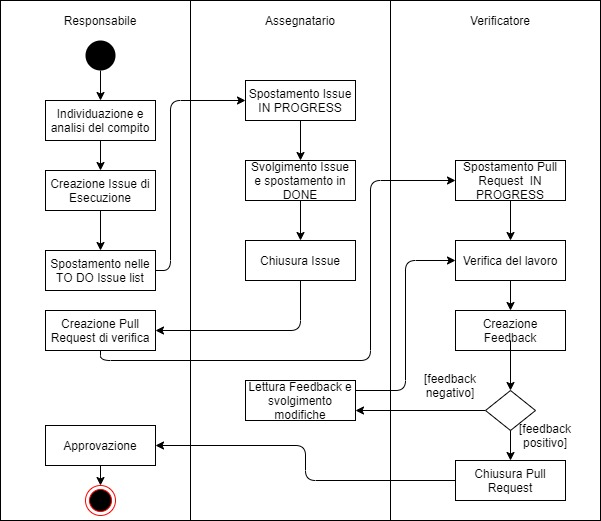
\includegraphics[scale=0.35]{res/images/ciclo_vita_ticket.jpg}
    \caption{Ciclo di vita di un ticket}
\end{figure}
Il ciclo di vita di un singol ticket interessa tre figure:
\begin{itemize}
    \item \textbf{Responsabile di progetto}: individua i compiti da svolgere, e una volta eseguiti e verificati li approva;
    \item \textbf{Assegnatario}: si prende in carico un ticket (o gliene viene incaricata una dal responsabile), la svolge, ed a lavoro terminato crea una pull request incaricando un soggetto per effettuare la verifica;
    \item \textbf{Verificatore}: controlla e verifica il lavoro che è stato svolto, dopo di che creerà un feedback all'interno della pull request con le correzioni da svolgere nel caso ce ne siano, altrimenti segnalerà completata la pull request e il lavoro in essa contenuto.
\end{itemize}

Le fasi del ciclo di vità di un ticket sono qui spiegate nel dettaglio.
\begin{itemize}
    \item \textbf{Individuazione del compito}: dopo aver rilevato nuove necessità, il responsabile di progetto le identifica come richieste da soddisfare creando appunto un nuovo compito. Ne valuta la complessità ed eventualmente lo suddivide in compiti più piccoli. Per ognuno determina una data di scadenza e se lo ritiene necessario può individuare uno o più assegnatari.
    \item \textbf{Creazione issue di esecuzione}: il responsabile crea una issue su GitHub secondo quanto riportato in \S\ref{_gestioneDeiCambiamenti}. Provvede ad inserire nella descrizione la data di scadenza precedentemente stabilità, ed eventualmente una breve descrizione del lavoro da svolgere.
    \item \textbf{Spostamento issue in "TO-DO"}: il responsabile sposta la issue nella colonna "TO-DO" all'interno della board di progetto, così da identificarla come da svolgere.
    \item \textbf{Spostamento issue in "IN PROGRESS"}: una volta che un assegnatario decide di iniziare il lavoro dopo essersi autoassegnato la issue, o dopo che il responsabile di progetto gli abbia incaricato l'attività, provvederà a spostarla nella colonna "IN PROGRESS".
    \item \textbf{Spostamento issue in "DONE"}: terminato il lavoro l'assegnatario provvederà a spostare la issue in "DONE" ed a chiudere la issue.
    \item \textbf{Creazione pull request}: il responsabile a questo punto dovrà creare una pull request dal ramo contenente il lavoro svolto al ramo dove dovranno essere applicate queste modifiche. Dovrà poi indicare nel campo "reviewer" un componente incaricato della verifica ed inserire la label "da revisionare". Può aggiungere alla pull request una descrizione contenente dei commenti sul lavoro svolto se ritiene che ciò possa essere utile al controllo da parte del verificatore. Conclude inserendo la pull request all'interno della sezione "TO-DO" della board di progetto.
    \item \textbf{Spostamento pull request in "IN PROGRESS"}: il verificatore quando inizia il lavoro di verifica sposta la pull request in "IN PROGRESS".
    \item \textbf{Creazione feedback di verifica}: terminata la verifica il verificatore scrive un feedback del lavoro sottopostogli, e richiede delle modifiche nel caso riscontri delle correzioni da fare. In questo caso assegna la pull request al componente del gruppo che l'ha creata, e modifica la label in "da correggere".
    \item \textbf{Svolgimento modifiche}: l'assegnatario dopo aver ricevuto dal verificatore un feedback sulle cose da sistemare provvederà a svolgerle. Una volta terminate le correzioni richiederà un'ulteriore verifica attraverso il tasto "re-reviews" e modificherà la label in "da revisionare".
    \item \textbf{Spostamento pull request in "DONE"}: se il verificatore non riscontra correzioni da fare, o quelle effettuate sono soddisfacenti, effettua il merge sul develop selezionando l'opzione "Squash and merge" e assegnare un titolo significativo al commit. Infine sposta la pull request in "DONE".
    \item \textbf{Approvazione del lavoro}: il responsabile di progetto dopo aver esaminato il lavoro lo approverà successivamente effettuando una pull request al ramo master.
\end{itemize}
\paragraph{Metriche di processo}
Per poter monitorare adeguatamente la pianificazione di risorse, tempi e costi del progetto vengono utilizzate le seguenti metriche:
\begin{itemize}
    \item \hyperref[_MPR-1]{\textbf{MPR-1:} Budgeted Cost of Work Scheduled (BCWS)};
    \item \hyperref[_MPR-2]{\textbf{MPR-2:} Actual Cost of Work Performed (ACWP)};
    \item \hyperref[_MPR-3]{\textbf{MPR-3:} Budgeted Cost of Work Performed (BCWP)};
    \item \hyperref[_MPR-4]{\textbf{MPR-4:} Cost Variance (CV)};
    \item \hyperref[_MPR-5]{\textbf{MPR-5:} Schedule Variance (SV)}.
\end{itemize}
Esse sono descritte più nel dettaglio in \S\ref{_metricheprocesso}

\subsection{Gestione dell'Infrastruttura} \label{_gestioneInfrastruttura}
\subsubsection{Scopo}
Il processo di gestione dell’infrastruttura permette di stabilire e mantenere un modello necessario per qualsiasi altro processo. Essa può includere hardware, software, strumenti, tecniche, standard e strutture per lo sviluppo.

\subsubsection{Descrizione}
Le prossime sezioni espongono gli strumenti impiegati dal gruppo SWException per quanto riguarda le attività di coordinamento e pianificazione del progetto. La lista presenterà i software utilizzati per tutte le comunicazioni e le conferenze del gruppo. Per ciascuno strumento viene fornita una breve descrizione e l'utilità all'interno dell'organizzazione dei lavori nel gruppo.

\subsubsection{Aspettative}
Con il processo di Gestione dell’Infrastruttura si ha l'obbiettivo di mantenere la coerenza dei componenti sia di codice che di documentazione, rendendoli disponibili a chiunque all'interno del gruppo. Gli strumenti e le tecnologie utilizzate servono a migliorare l'esperienza lavorativa e le comunicazioni tra i componenti del gruppo.


\subsubsection{Per il Coordinamento}
Di seguito viene presentata una breve descrizione degli strumenti utilizzati.

\paragraph{Slack}
Slack è uno strumento collaborativo aziendale, utilizzato per inviare messaggi in modo istantaneo ai membri di un preciso team di lavoro. L’applicativo permette ad un utente di iscriversi
a diversi workspace. Per ogni workspace di appartenenza è concessa la creazione di canali
tematici dove sviluppare delle conversazioni specializzate. Ciò permette di evitare la trattazione di diversi argomenti su un’unica chat generale, come invece avviene in Telegram. Per questo è stato deciso dal gruppo di utilizzare Slack per le comunicazioni ufficiali e per la suddivisione del workspace in canali relativi ai vari ambi da trattare. Slack può inoltre venire integrato con diverse applicazioni come Google Calendar, Outlook Calendar e GitHub. Oltre all'utilizzo per comunicazioni interne la piattaforma verrà utilizzata per comunicare col proponente del progetto.

\paragraph{Telegram}
Telegram è uno strumento di messaggistica istantanea molto utilizzato per la creazione e gestione di gruppi e canali. Fin dal primo giorno di incontro e presentazione digitale, è sempre stato lo strumento più utilizzato per le decisioni e le discussioni relative a qualsiasi ambito del progetto. Il gruppo ha quindi deciso di utilizzare Telegram insieme a Slack come strumenti per la comunicazione interna.

\paragraph{Zoom}
Zoom è un servizio di videocall e chat online che tramite una piattaforma software peer-to-peer viene utilizzata per conferenze e lavoro. È stato utilizzato come primo strumento per le videoconferenze del gruppo. È uno strumento facile da utilizzare e come tutti i servizi di meeting permette di condividere lo schermo. Permette di registrare le videoconferenze e di condividerle tra i partecipanti attraverso un link. Sono state create dal gruppo delle coordinate, accessibili attraverso un link zoom appuntato sulla chat di Telegram, per le videochiamate in modo da semplificare la gestione delle stesse e per permettere ai partecipanti di avere una stanza comune per discutere.

\paragraph{Outlook}
\glock{Outlook} è un'app Web e mobile di gestione delle informazioni personali di Microsoft composta da servizi di posta Web, calendario, contatti e attività. È stata utilizzata dal gruppo per la creazione di una email comune a tutti i partecipanti a rappresentanza dei \textit{SWException}.

\paragraph{GitHub}
GitHub è un sito Web e un servizio basato su cloud che aiuta gli sviluppatori a memorizzare e gestire il proprio codice, nonché a tracciare e controllare le modifiche al proprio codice. GitHub è essenzialmente sviluppato su due principi connessi tra di loro:
\begin{itemize}
    \item controllo versioni;
    \item \textit{Git}.
\end{itemize}
Il controllo della versione aiuta il gruppo a tenere traccia e gestire le modifiche al codice di un progetto software. Man mano che un progetto software cresce, il controllo della versione diventa essenziale per il completamento dei requisiti. Il controllo della versione consente agli sviluppatori di lavorare in sicurezza attraverso \glock{Branch} e \glock{Merge}. Il Branch duplica parte del codice sorgente (chiamato repository). Ogni componente del gruppo può quindi apportare modifiche in modo sicuro a quella parte del codice senza influire sul resto del progetto. Una volta che lo sviluppatore ottiene che la sua parte di codice funzioni correttamente, può unire nuovamente quel codice nel codice sorgente principale per renderlo ufficiale. Il processo di unione è definito merge.
Git è invece un sistema di controllo della versione distribuito: l'intera base di codice e la cronologia sono disponibili sul computer di ogni sviluppatore, il che consente facili branch e merge.

\paragraph{Google Meet}
\glock{Google Meet} è una piattaforma per videocall e conferenze simile a Zoom. Permette di gestire i video meeting attraverso link d'invito e salvataggio sul calendario. È stato utilizzato dal gruppo per le comunicazioni esterne con il proponente.

\paragraph{Issue Tracking System}
L'\glock{Issue Tracking System} di GitHub è un ottimo strumento per tenere traccia di attività, miglioramenti e bug per quanto riguarda il progetto. Il gruppo utilizzerà questo sistema per gestire l'avanzamento del software, i compiti assegnati ad ogni componente, le milestone e la verifica del codice.

\subsubsection{Per la Pianificazione}
Di seguito viene invece esposto lo strumento utilizzato per pianificare le attività da svolgere.
\paragraph{GanttProject}
Per il supporto all’attività di pianificazione del progetto e per la realizzazione di diagrammi è stato deciso di utilizzare \glock{GanttProject}, software open-source e multi-piattaforma. Esso permette di visualizzare su una linea temporale la pianificazione delle attività, potendo visualizzare quelle che possono essere svolte in parallelo oltre che la dipendenza temporale tra esse.

\subsection{Miglioramento del processo} \label{_miglioramentoDelProcesso}
\subsubsection{Scopo}
Il processo di Miglioramento permette di controllare le dinamiche relative al progetto con l'intento di migliorare l'efficacia e l'efficienza dei suoi processi.
\subsubsection{Descrizione}
Ciascun processo sarà monitorato da chi di dovere durante tutto il ciclo di vita del software. Il gruppo si pone l'obbiettivo di seguito la Pianificazione affiancandola allo sviluppo controllato dei componenti che compongono il software. Il giusto equilibrio tra pianificazione e controllo dello sviluppo sarà un punto fondamentale per il raggiungimento degli obbiettivi fissati. Per assicurare l'efficienza e l'efficacia dei processi verrà eseguita una loro revisione a intervalli appropriati in modo da confermare e conservare il lavoro svolto in precedenza. Il gruppo dovrà poi definire i miglioramenti necessari e attuarli in maniera adeguata nella revisione del processo in questione. I dati e gli storici saranno raccolti e analizzati nel piano di qualifica per scovare eventuali problematiche e individuare i punti di forza dei processi impiegati. L'analisi deve essere usata come feedback per migliorare i processi, raccomandando modifiche da applicare alle procedure, agli strumenti e all'utilizzo delle tecnologie.

\subsection{Formazione del personale} \label{_formazione}
\subsubsection{Scopo}
Il Processo di Formazione permette di avere e mantenere nel tempo personale competente. I membri del gruppo \textit{SWException} sono tenuti a formarsi individualmente sulle tecnologie richieste per il completamento del progetto e, nel caso di incomprensioni o chiarimenti nell'utilizzo di esse, il proponente si è dichiarato disponibile ad organizzare consultazioni video dopo opportune ricerche autonome.
\subsubsection{Descrizione}
Ciascun membro del gruppo deve provvedere alla propria formazione autonomamente,
studiando le tecnologie usate e colmando eventuali carenze. In particolare, i soggetti in
deficit dovranno colmare le loro mancanze approfondendo lo studio personale; sarà compito
dei membri più esperti condividere le conoscenze per operare secondo il principio del miglioramento continuo.
Il team farà riferimento alla documentazione di seguito esposta, oltre a quella reperita per
proprio conto.

\subsubsection{Metriche}
Per la formazione del personale non si fa uso di particolari metriche di qualità.

\subsubsection{Attività}
Ciò che ci si attende da tale processo è di poter assicurare una qualità del lavoro che
rispetti le aspettative, grazie alla presenza di personale competente in grado di
svolgere i compiti assegnati. In questa sezione sono elencate le tecnologie e i linguaggi di programmazione necessari per lo svolgimento del capitolato con i relativi link al sito ufficiale.

\paragraph{Linguaggi di Programmazione}
\begin{itemize}
    \item \textbf{\glock{Typescript}}: \url{https://www.typescriptlang.org/};
\end{itemize}
\paragraph{Tecnologie}
\begin{itemize}
    \item \textbf{\glock{Serverless}}: \url{https://www.serverless.com/};
    \item \textbf{\glock{Next.js}}: \url{https://nextjs.org/};
    \item \textbf{\textit{Latex}}: \url{https://www.latex-project.org/help/documentation/};
    \item \textbf{\textit{Git}}: \url{https://git-scm.com/doc};
    \item \textbf{\textit{GitHub}}: \url{https://docs.github.com/en/free-pro-team@latest/github};
    \item \textbf{\glock{AWS Lambda}}: \url{https://aws.amazon.com/it/lambda/?nc2=h_ql_prod_fs_lbd};
    \item \textbf{\glock{AWS DynamoDB}}: \url{https://aws.amazon.com/it/dynamodb/?nc2=h_ql_prod_db_ddb};
    \item \textbf{\glock{AWS API Gateway}}: \url{https://aws.amazon.com/api-gateway/?nc2=type_a};
    \item \textbf{\glock{AWS S3}}: \url{https://aws.amazon.com/s3/?nc2=type_a};
    \item \textbf{\glock{Amazon CloudWatch}}: \url{https://aws.amazon.com/cloudwatch/?nc2=type_a};
    \item \textbf{\glock{Auth0}}: \url{https://auth0.com/#!}.
\end{itemize}